\chapter{Algorithm Overview}

\section{Base Algorithm}

Let's describe the base algorithm of this thesis for multi-tenant caching, its detailed 
pseudcode is shown in Figure \ref{fig:base_algorithm}.

For each page access, the algorithm first checks if the page is in the cache,
in case it is, it returns the buffer location and the hit flag as true. It also 
updates the access history of the page in the cache eviction policy, for example,
for LRU, it moves the page to the top of the list (of that tenant).

If the page is not in the cache, the algorithm checks if there is available space
in the cache. If there is, it gets the first available buffer location and adds the
page to the cache. 

If there is no available space, the algorithm selects a page to evict from the cache 
using the tenant selection policy and the cache eviction policy. The algorithm then 
evicts the page and adds the new page to the cache.

Note that the tenant selection policy's responsibility is to select the tenant to evict
from the cache, each time a page needs to be evicted, for this, some metrics of the 
tenants can be used.

The cache eviction policy's responsibility is to manage the cache, including:
\begin{itemize}
    \item \textbf{UpdateAccessHistory}(\textit{page}, \textit{tenant}): Update the access history when a page is accessed.
    \item \textbf{AddPageToCache}(\textit{page}, \textit{tenant}, \textit{buffer\_location}): Add a page to the cache of a tenant in a specific buffer location.
    \item \textbf{EvictPage}(\textit{tenant\_to\_evict}): Evict a page from the cache of a tenant.
\end{itemize}

Each of the described tenant selection policies and cache eviction policies will implement
these functions, and the base algorithm will call them when needed.

Note that the base algorithm is a general dynamic multi-tenant cache algorithm that can 
be used with different tenant selection and cache eviction policies. The next sections 
will describe the tenant selection and cache eviction policies used with the base algorithm.

Another algorithm for dynamic multi-tenant buffer allocation was proposed in the 
literature in \cite{buffer-sharing-1}, a hybrid approach combining global and static 
buffer allocation was proposed in \cite{article-for-2level-forecasting}.

\begin{figure}[htbp]
    \centering
    \begin{minipage}{\linewidth}
    \begin{algorithm}[H]
        \caption{Base Algorithm to process each page access}
        \begin{algorithmic}
            \STATE \textbf{Input:} $(p, t)$ - The page id and tenant of the page to be accessed.
            \STATE \textbf{Output:} $(b, h)$ - The buffer location of the page accessed and whether it is a hit or not.
            \STATE
            \STATE $(\text{buffer\_location}, \text{is\_hit}) \leftarrow \text{GetPageLocationIfItIsInCache}(\text{page} = p, \text{tenant} = t)$
            \IF {$\text{is\_hit}$}
                \STATE $\text{CacheEvictionPolicy.UpdateAccessHistory}(\text{page} = p, \text{tenant} = t)$
                \RETURN $(b = \text{buffer\_location}, h = \textbf{true})$
            \ELSE
                \STATE \COMMENT {Page is not in cache, we need to find a place for it}
                \IF {There is available space in cache}
                    \STATE $\text{available\_location} \leftarrow \text{GetAvailableBufferLocation}()$ \COMMENT {Get the first available buffer location}
                    \STATE $\text{CacheEvictionPolicy.AddPageToCache(\text{page} = p, \text{tenant} = t, \text{available\_location})}$
                    \RETURN $(b = \text{available\_location}, h = \textbf{false})$
                \ELSE
                    \STATE \COMMENT {Cache is full, we need to evict a page}
                    \STATE $\text{tenant\_to\_evict} \leftarrow \text{TenantSelectionPolicy.GetTenantToEvict}()$
                    \STATE $\text{evicted\_page} \leftarrow \text{CacheEvictionPolicy.EvictPage}(\text{tenant\_to\_evict})$
                    \STATE $b \leftarrow \text{evicted\_page.buffer\_location}$
                    \STATE $\text{CacheEvictionPolicy.AddPageToCache}(\text{page} = p, \text{tenant} = t, \text{buffer\_location} = b)$
                    \RETURN $(b, h = \textbf{false})$
                \ENDIF
            \ENDIF
            \STATE
            \STATE \textbf{function} GetPageLocationIfItIsInCache(page, tenant):
            \STATE \hspace{\algorithmicindent} \textbf{if} page is in cache \textbf{then}
            \STATE \hspace{\algorithmicindent} \hspace{\algorithmicindent} \textbf{return} $(\text{page.buffer\_location}, \textbf{true})$
            \STATE \hspace{\algorithmicindent} \textbf{else}
            \STATE \hspace{\algorithmicindent} \hspace{\algorithmicindent} \textbf{return} $(\textbf{null}, \textbf{false})$
            \STATE \hspace{\algorithmicindent} \textbf{end if}
            \STATE \textbf{end function}
        \end{algorithmic}
    \end{algorithm}
    \caption{Base Algorithm}
    \label{fig:base_algorithm}
    \end{minipage}
\end{figure}
    

\section{Tenant Selection Policy}

The tenant selection policy is responsible for selecting the tenant
to evict from the cache when a page needs to be evicted.

In order to properly select the tenant to evict, the tenant selection policies will use 
some metrics of the tenants, such as the number of pages currently in the cache, 
the number of accesses, the number of hits, the number of faults. It is simple to 
keep track of these metrics with negligible overhead. In many applications, these 
metrics are already kept track of in the cache eviction policy, like in many DBMSs \cite{buffer-sharing-1}.

Other important metric that will allow us to better select the tenant to evict is 
the number of hits or faults if we had a cache of the promised size, or a cache 
$x\%$ higher than the recommendation in case there is no promised size, keeping track of 
this metrics requires additional overhead, like to simulate a LRU or other cache 
of the promised size for each tenant. Simulating a cache per tenant for selection 
purposes has been proposed and analysed in the literature in \cite{buffer-sharing-1}.

Many of the tenant selection policies described here will require aditional overhead 
metrics in order to work properly, in real applications, this overhead needs to be 
considered in comparison to the benefits of the eviction policy.

\subsection{Fault Ratio Policy}

Fault ratio policy comes from the idea that the tenant with the highest fault ratio
with respect to the fault ratio of the cache of the promised size (or size $x\%$ bigger than
the recommendation) should be evicted.

The evicted tenant $t$ is the one that minimizes the following formula:

$$
\left( \frac{\text{Solution Cache faults}_t - \text{LRU Cache faults}_t}{\text{LRU Cache faults}_t} \right) ^2 \text{Priority}_t \, \cdot \, \text{sgn}( \text{Solution Cache faults}_t - \text{LRU Cache faults}_t )
$$

Where:

\begin{itemize}
    \item $\text{Solution Cache faults}_t$ --- is the number of faults of the tenant in the cache of the promised size (or $x\%$ bigger than the recommendation).
    \item $\text{LRU Cache faults}_t$ --- is the number of faults of the tenant in a LRU cache of the promised size (or $x\%$ bigger than the recommendation).
    \item $\text{Priority}_t$ --- is the priority of the tenant.
    \item $\text{sgn}(x)$ --- is the sign function, returning $1$ if $x > 0$, $-1$ if $x < 0$ and $0$ if $x = 0$.
\end{itemize}

Note that we evict from the tenant that is performing the best in terms of our penalty
function, we use sign instead of condition to penalize by how much the tenant is performing
better than the LRU cache of the promised size, so we evict more from tenants that are
performing better.

This policy is a part of the policy proposed by Noé Weeks in \cite{noe-weeks-comments} for 
ICPC 2023 Online Spring Challenge powered by Huawei: Buffer Sharing in Multi-Tenant Database Environment \cite{huawei-challenge}.

Note that this tenant selection policy requires additional overhead to keep track of the
number of faults of the tenants in the cache of the promised size (or $x\%$ bigger than the recommendation),
so it needs to simulate an LRU cache for each tenant.

This policy can be modified to use as baseline algorithm to compare, the same cache algorithm
that will be used in the cache eviction policy, in order to use it as a quantitative measure 
of the impact of multi-tenancy on performance. We did not do this in this thesis, since
our penalty function is based on the LRU cache of the promised size.

\subsection{Hit Ratio Policy}

Hit ratio policy is very similar to the fault ratio policy, but instead of using the faults,
it uses the hits of the tenants in the cache of the promised size (or $x\%$ bigger than the recommendation).

The evicted tenant $t$ is the one that minimizes the following formula:

$$
\left( \frac{\text{LRU Cache hits}_t - \text{Solution Cache hits}_t}{\text{LRU Cache hits}_t} \right) ^2 \text{Priority}_t \, \cdot \, \text{sgn}( \text{LRU Cache hits}_t - \text{Solution Cache hits}_t )
$$

Where:

\begin{itemize}
    \item $\text{Solution Cache hits}_t$ --- is the number of hits of the tenant in the cache of the promised size (or $x\%$ bigger than the recommendation).
    \item $\text{LRU Cache hits}_t$ --- is the number of hits of the tenant in a LRU cache of the promised size (or $x\%$ bigger than the recommendation).
    \item $\text{Priority}_t$ --- is the priority of the tenant.
    \item $\text{sgn}(x)$ --- is the sign function, returning $1$ if $x > 0$, $-1$ if $x < 0$ and $0$ if $x = 0$.
\end{itemize}

This policy is very similar to the fault ratio policy, since more hits means less faults,
and we observed better results with the fault ratio policy, therefore we will use it more.

Like in the fault ratio policy, this policy requires additional overhead to keep track of the
number of hits of the tenants in the cache of the promised size (or $x\%$ bigger than the recommendation),
so it needs to simulate an LRU cache for each tenant.

This policy can also be modified to use as baseline algorithm to compare, the same cache algorithm
that will be used in the cache eviction policy, in order to use it as a quantitative measure
of the impact of multi-tenancy on performance.

\subsection{Fault Ratio with Cache Used Policy}

Fault ratio with cache used policy is a modification of the fault ratio policy, where we
divide by the ratio squared of the cache currently used by the tenant and the cache of the
promised size (or $x\%$ bigger than the recommendation).

The evicted tenant $t$ is the one that minimizes the following formula:

$$
\frac{ \left( \frac{\text{Solution Cache faults}_t - \text{LRU Cache faults}_t}{\text{LRU Cache faults}_t} \right) ^2 \text{Priority}_t \, \cdot \, \text{sgn}( \text{Solution Cache faults}_t - \text{LRU Cache faults}_t ) }{ \left( \frac{\text{Cache Used}_t}{\text{LRU Base Cache Size}_t} \right) ^2 }
$$

Where:

\begin{itemize}
    \item $\text{Solution Cache faults}_t$ --- is the number of faults of the tenant in the cache of the promised size (or $x\%$ bigger than the recommendation).
    \item $\text{LRU Cache faults}_t$ --- is the number of faults of the tenant in a LRU cache of the promised size (or $x\%$ bigger than the recommendation).
    \item $\text{Priority}_t$ --- is the priority of the tenant.
    \item $\text{sgn}(x)$ --- is the sign function, returning $1$ if $x > 0$, $-1$ if $x < 0$ and $0$ if $x = 0$.
    \item $\text{Cache Used}_t$ --- is the number of pages currently in the cache of the tenant.
    \item $\text{LRU Base Cache Size}_t$ --- is the size of the LRU cache of the promised size (or $x\%$ bigger than the recommendation) for the tenant.
\end{itemize}

The modification in this policy comes from the idea that if a tenant is using more cache
with respect to the cache of the promised size, it can match the base LRU performance 
better, so we can afford to evict more from this tenant, in the same way, if a tenant is
using less cache, it will be harder to match the base LRU performance, so we should evict
less from this tenant.

This policy requires same overhead as the fault ratio policy, since it needs to keep track
the same metrics plus the cache used by the tenants, which is a simple metric to keep track
of.

It can also be modified to use as baseline algorithm to compare, the same cache algorithm
that will be used in the cache eviction policy, in order to use it as a quantitative measure
of the impact of multi-tenancy on performance.

This policy showed the better results when we tried, therefore we will use it as the main 
tenant selection policy in this thesis, it was also used as the main tenant selection policy
by Noé Weeks \cite{noe-weeks-comments} in the ICPC 2023 Online Spring Challenge powered by Huawei: Buffer Sharing in
Multi-Tenant Database Environment \cite{huawei-challenge}.

\subsection{Naive Policy}

For the naive policy, we will evict from the tenant that its cache size is furthest
from the cache of the promised size (or $x\%$ bigger than the recommendation) (in ratio).

The evicted tenant $t$ is the one that minimizes the following formula:

$$
\frac{ \text{Cache Used}_t }{ \text{LRU Base Cache Size}_t }
$$

In case of a tie (each tenant has the number of pages in the cache with the same 
proportion to the recommendation), we will evict from the same tenant of the page that 
is being accessed.


In case of not changing recommendation, like in the case of comparing to the cache of
the promised size, this policy makes our algorithm behave like a static cache algorithm
for each tenant.

This policy requires no additional overhead, since it only needs to keep track of the
number of pages in the cache of the tenants.

\section{Cache Eviction Policy}

The cache eviction policy is responsible for managing the cache, including updating the
access history when a page is accessed, adding a page to the cache and evicting a page
from the cache.

The cache eviction policies will be used with the base algorithm, and they will implement
the following functions:

\begin{itemize}
    \item \textbf{UpdateAccessHistory}(\textit{page}, \textit{tenant}): Update the access history when a page is accessed.
    \item \textbf{AddPageToCache}(\textit{page}, \textit{tenant}, \textit{buffer\_location}): Add a page to the cache of a tenant in a specific buffer location.
    \item \textbf{EvictPage}(\textit{tenant\_to\_evict}): Evict a page from the cache of a tenant.
\end{itemize}

Note that the cache eviction policies need to be implemented in a different way with respect
to the single tenant cache problem, since here we can evict a page from one tenant, and 
use the freed space to add a page from another tenant, and the size assigned to each tenant
can change over time.

In the implementations, we will keep a separate structure of cache
for each tenant, like a separated linked list for each tenant in the case of LRU,
note that, however, buffer locations are shared between tenants, so we can evict a page
from one tenant and use the freed space to add a page from another tenant.

Since in this thesis we are focusing on the cache eviction and the tenant selection 
policies we will not keep cache items or pages themselves in the cache, we will just keep
the buffer location in the cache. 

Let's describe each of the cache eviction policy in detail in next sections.

\subsection{LRU}

Least Recently Used (Belady, 1966), is a cache eviction policy that evicts the page that was least
recently used, it comes from the assumption that the page that was least recently used is the
least likely to be used in the near future.

It was the was the algorithm of choice in the most cases until the early 80s \cite{2q-article},
and it is the cache eviction policy that has been studied the most and it is considered
the most predictable cache eviction policy \cite{lru-analysis-article}, and it never
replaces more than a factor of $B$ as many elements as the optimal offline algorithm, where $B$
is the size of the buffer \cite{lru-factor-b}. For example, LRU on a buffer of size $B$ will
never replace more than twice as many elements as the optimal or clairvoyant algorithm on a 
buffer of size $B/2$ \cite{2q-article}.

This eviction policy is usually implemented with a doubly linked list to keep track of the
access history of the pages and a hash table or array to keep track of the buffer location
of the pages, so it can process each page access in $O(1)$ time.

For LRU cache, we can implement each of the functions as follows:

\begin{itemize}
    \item \textbf{UpdateAccessHistory}(\textit{page}, \textit{tenant}): Move the page to the top of the list of the tenant.
    \item \textbf{AddPageToCache}(\textit{page}, \textit{tenant}, \textit{buffer\_location}): Add the page to the top of the list of the tenant.
    \item \textbf{EvictPage}(\textit{tenant\_to\_evict}): Evict the page from the bottom of the list of the tenant.
\end{itemize}

\begin{figure}[htbp]
    \centering
    \begin{minipage}{\linewidth}
    \begin{algorithm}[H]
        \caption{LRU Cache Eviction Policy}
        \begin{algorithmic}
            \STATE \textbf{function} UpdateAccessHistory(page, tenant):
            \STATE \hspace{\algorithmicindent} CacheList[tenant].\textbf{move\_to\_top}(CacheLocations[tenant][page])
            \STATE \hspace{\algorithmicindent} CacheLocations[tenant][page] = CacheList[tenant].\textbf{head}
            \STATE \textbf{end function}
            \STATE
            \STATE \textbf{function} AddPageToCache(page, tenant, buffer\_location):
            \STATE \hspace{\algorithmicindent} CacheList[tenant].\textbf{add\_to\_top}(page)
            \STATE \hspace{\algorithmicindent} CacheLocations[tenant][page] = CacheList[tenant].\textbf{head}
            \STATE \textbf{end function}

            \STATE
            \STATE \textbf{function} EvictPage(tenant\_to\_evict):
            \STATE \hspace{\algorithmicindent} page = CacheList[tenant\_to\_evict].\textbf{remove\_from\_tail}()
            \STATE \hspace{\algorithmicindent} CacheLocations[tenant][page] = \textbf{null}
            \STATE \hspace{\algorithmicindent} \textbf{return} page
            \STATE \textbf{end function}
        \end{algorithmic}
    \end{algorithm}
    \caption{LRU Cache Eviction Policy}
    \label{fig:lru}
    \end{minipage}
\end{figure}

CacheList is a doubly linked list per tenant, that keeps the pages in the cache,
in the order of the access history, the head of the list is the most recently used
page.

CacheLocations is a hash map or array that keeps the location of the pages in the cache,
so we can process each page access in $O(1)$ time.

\subsection{LFU}

Least Frequently Used (LFU) \cite{wikipedia-lfu} is a cache eviction policy that evicts
the page that was least frequently used, and if there is a tie (two or more pages have
the same frequency of use), it evicts the page that was least recently used. 
\cite{cache-management-algorithms-for-flexible-filesystems}

It is based on the idea that the pages accessed most frequently are the most likely 
to be accessed in the near future. 

When the probability distribution of the data access pattern is constant over time, LFU 
yields the highest performance \cite{lfu-highest-perf-zipf} \cite{lfu-highest-perf-inproc} \cite{tiny-lfu},
but in most practical workloads, the access frequency changes radically over time. For
example, in a video caching service; a video clip that is really popular on a 
given day might not be accessed a few days later. Hence, there is no point in 
keeping that item in cache once its popularity has faded just because it was once very 
popular \cite{tiny-lfu}.

In the ideal LFU, we would keep a counter of the number of accesses of each page,
even if the page is not in the cache, but this is not practical in real applications,
since it requires memory proportional to the number of pages accessed, therefore, in 
practice, frequency counter is kept in the cache, and it is forgotten when the page is
evicted \cite{wikipedia-lfu}.

Single tenant LFU can be implemented in $O(1)$ time \cite{o-1-lfu}, but it needs to keep
track of the frequency of the least frequently used page, and to keep this efficiently,
it relies on the fact that each time a page is evicted, a new page is added to the cache,
so it can update the frequency of the least frequently used page easily, but in multi-tenant
caching, we can evict a page from one tenant and add a page from another tenant, so we would
need to keep track of the frequency of the least frequently used page for each tenant in a
different way, which is not practical.

Due to this, we can not implement LFU in multi-tenant caching in $O(1)$ time, we would need
to use then a heap to keep track of the frequency of the pages, and a hash map or array to 
keep track of the locations of the pages, so we can implement LFU in multi-tenant caching 
in $O(\log n)$ time, where $n$ is the number of pages in the cache.

For LFU cache, we can implement each of the functions as follows:

\begin{itemize}
    \item \textbf{UpdateAccessHistory}(\textit{page}, \textit{tenant}): Increase the frequency of the page in the cache of the tenant, and update the heap.
    \item \textbf{AddPageToCache}(\textit{page}, \textit{tenant}, \textit{buffer\_location}): Add the page to the heap of the tenant, with the frequency of 1.
    \item \textbf{EvictPage}(\textit{tenant\_to\_evict}): Evict the page with the least frequency from the heap of the tenant.
\end{itemize}

\begin{figure}[htbp]
    \centering
    \begin{minipage}{\linewidth}
    \begin{algorithm}[H]
        \caption{LFU Cache Eviction Policy}
        \begin{algorithmic}
            \STATE \textbf{function} UpdateAccessHistory(page, tenant):
            \STATE \hspace{\algorithmicindent} pageInHeap = CacheLocations[tenant][page]
            \STATE \hspace{\algorithmicindent} pageInHeap.frequency += 1
            \STATE \hspace{\algorithmicindent} CacheLocations[tenant][page] = pageInHeap
            \STATE \hspace{\algorithmicindent} CacheHeaps[tenant].\textbf{heapify}(pageInHeap)
            \STATE \textbf{end function}
            \STATE
            \STATE \textbf{function} AddPageToCache(page, tenant, buffer\_location):
            \STATE \hspace{\algorithmicindent} pageInHeap = \textbf{new} PageInHeap(page = page, frequency = 1, buffer\_location = buffer\_location)
            \STATE \hspace{\algorithmicindent} CacheHeaps[tenant].\textbf{insert}(pageInHeap)
            \STATE \hspace{\algorithmicindent} CacheLocations[tenant][page] = pageInHeap
            \STATE \textbf{end function}

            \STATE
            \STATE \textbf{function} EvictPage(tenant\_to\_evict):
            \STATE \hspace{\algorithmicindent} page = CacheHeaps[tenant\_to\_evict].\textbf{extract\_min}()
            \STATE \hspace{\algorithmicindent} CacheLocations[tenant][page] = \textbf{null}
            \STATE \hspace{\algorithmicindent} \textbf{return} page
            \STATE \textbf{end function}
        \end{algorithmic}
    \end{algorithm}
    \caption{LFU Cache Eviction Policy}
    \label{fig:lfu}
    \end{minipage}
\end{figure}

CacheHeaps is a min heap per tenant, that keeps the pages in the cache, in the order of the
frequency of the pages, the root of the heap is the page with the least frequency.

CacheLocations is a hash map or array that keeps the location of the pages in the cache,
so we can process each page access in $O(1)$ time.

\subsection{LRU-2}

LRU-2 is a generalization of LRU, where LRU is LRU-1, and it is a special case of LRU-k, 
where $k = 2$. It is a cache eviction policy whose idea is to keep track of 
the second most recent refence of each page, using this information to estimate the 
inter-reference time of each page \cite{lru-k}.

Unlike LRU, LRU-2 is scan resistant, since it gives low priority to pages that have been 
scanned or to pages that belong to a big randomly accessed file \cite{2q-article}, and it 
does not suffer so much from access pattern changes like LFU, because of the correlated 
reference period \cite{lru-k}.

Correlated references are references that are close to each other in time, it has been 
shown that they are common in real workloads. They have been described in the literature 
\cite{lru-k} \cite{2q-article} \cite{lrfu-article}.

In order to handle the correlated references, and to be more resistant to access pattern 
changes, LRU-2 has a tunable parameter, the Correlated Reference Period, which is the
time window or number of references that are considered to be correlated.

LRU-2 evicts the page that has the smallest second-to-last access time, among the pages
that are not in the Correlated Reference Period.

In LRU-2, there is a need of keeping in memory a history of pages that are not in the 
cache, for example, if a page $p$ is accessed, it's recorded and stored in a buffer. If 
$p$ wasn't accessed recently enough to remember, its second to last access will be 0, 
and it will be evicted. To prevent cycling $p$ in and out of memory without recognizing 
its frequent use, we retain its access history for a while after its last access, this is 
called the Retained Information Period \cite{lru-k} \cite{2q-article}.

In the literature \cite{lru-k} LRU-2 is proposed to be implemented in an asynchronous way,
with separate processes or threads to handle pages that are no longer in the Correlated 
Reference Period, or pages that are no longer in the Retained Information Period, but in 
this thesis we will implement it in a synchronous, by defining the Correlated Reference
Period and the Retained Information Period in terms of the number of references.

Pages in the Correlated Reference Period will be handled in a FIFO list, pages in the cache
that are not in the Correlated Reference Period will be handled in a heap, since we need
to evict from these pages based on the second-to-last access time, pages in the Retained
Information Period could be handled with another heap to delete based on the second-to-last
access time, but to avoid additional overhead, since LRU-2 is already complex, we will
handle them in a FIFO list without affecting the performance of the algorithm too much
(note that using this, they will be evicted based on the time they were removed from the 
cache, but since this pages are not in the cache anymore, it will not affect much the performance
of the algorithm). 

For LRU-2 cache, we can implement each of the functions as follows:

\begin{itemize}
    \item \textbf{UpdateAccessHistory}(\textit{page}, \textit{tenant}): If the page is 
    in Correlated Reference Period, just update its last access time (do not update the 
    second-to-last access time, since it is a correlated reference), if the page is not 
    in the Correlated Reference Period, remove it from the heap, update its last and
    second-to-last access time, and add it to the front of the Correlated Reference 
    Period FIFO list, move last correlated page to the heap if needed.
    \item \textbf{AddPageToCache}(\textit{page}, \textit{tenant}, \textit{buffer\_location}): 
    Add the page to the front of the Correlated Reference Period FIFO list, move last 
    correlated page to the heap if needed.
    \item \textbf{EvictPage}(\textit{tenant\_to\_evict}): Evict the page on the top of 
    the heap (or from the FIFO list if the heap is empty), remove it and add it to the 
    Retained Information Period FIFO list, remove the last page from the Retained
    Information Period FIFO list if needed.
\end{itemize}

\begin{figure}[htbp]
    \centering
    \begin{minipage}{\linewidth}
    \begin{algorithm}[H]
        \caption{LRU-2 Cache Eviction Policy}
        \begin{algorithmic}
            \STATE \textbf{function} UpdateAccessHistory(page, tenant):
            \STATE \hspace{\algorithmicindent} \textbf{if} CRP\_Locations[tenant][page] != \textbf{null} \textbf{then}
            \STATE \hspace{\algorithmicindent} \hspace{\algorithmicindent} pageInCRP = CRP\_Locations[tenant][page]
            \STATE \hspace{\algorithmicindent} \hspace{\algorithmicindent} pageInCRP.last\_access = current\_time
            \STATE \hspace{\algorithmicindent} \textbf{else}
            \STATE \hspace{\algorithmicindent} \hspace{\algorithmicindent} page = HeapLocations[tenant][page]
            \STATE \hspace{\algorithmicindent} \hspace{\algorithmicindent} CacheHeaps[tenant].\textbf{remove}(page)
            \STATE \hspace{\algorithmicindent} \hspace{\algorithmicindent} HeapLocations[tenant][page] = \textbf{null}
            \STATE \hspace{\algorithmicindent} \hspace{\algorithmicindent} page.second\_to\_last\_access = page.last\_access
            \STATE \hspace{\algorithmicindent} \hspace{\algorithmicindent} page.last\_access = current\_time
            \STATE \hspace{\algorithmicindent} \hspace{\algorithmicindent} CRP\_List[tenant].\textbf{add\_to\_front}(page)
            \STATE \hspace{\algorithmicindent} \hspace{\algorithmicindent} CRP\_Locations[tenant][page] = CRP\_List[tenant].\textbf{head}
            \STATE \hspace{\algorithmicindent} \hspace{\algorithmicindent} \textbf{if} CRP\_List[tenant].\textbf{size}() $>$ CRP\_Size[tenant] \textbf{then}
            \STATE \hspace{\algorithmicindent} \hspace{\algorithmicindent} \hspace{\algorithmicindent} MoveLastPageInCRPToHeap(tenant)
            \STATE \hspace{\algorithmicindent} \hspace{\algorithmicindent} \textbf{end if}
            \STATE \hspace{\algorithmicindent} \textbf{end if}
            \STATE \textbf{end function}
            \STATE
            \STATE \textbf{function} AddPageToCache(page, tenant, buffer\_location):
            \STATE \hspace{\algorithmicindent} \textbf{if} RIP\_Locations[tenant][page] != \textbf{null} \textbf{then}
            \STATE \hspace{\algorithmicindent} \hspace{\algorithmicindent} pageInRIP = RIP\_Locations[tenant][page]
            \STATE \hspace{\algorithmicindent} \hspace{\algorithmicindent} second\_to\_last\_access = pageInRIP.last\_access
            \STATE \hspace{\algorithmicindent} \hspace{\algorithmicindent} RIP\_List[tenant].\textbf{remove}(pageInRIP)
            \STATE \hspace{\algorithmicindent} \hspace{\algorithmicindent} RIP\_Locations[tenant][page] = \textbf{null}
            \STATE \hspace{\algorithmicindent} \textbf{else}
            \STATE \hspace{\algorithmicindent} \hspace{\algorithmicindent} second\_to\_last\_access = 0
            \STATE \hspace{\algorithmicindent} \textbf{end if}
            \STATE \hspace{\algorithmicindent} pageInCRP = \textbf{new} PageInCRP(page = page, last\_access = current\_time, second\_to\_last\_access = second\_to\_last\_access, buffer\_location = buffer\_location)
            \STATE \hspace{\algorithmicindent} CRP\_List[tenant].\textbf{add\_to\_front}(pageInCRP)
            \STATE \hspace{\algorithmicindent} CRP\_Locations[tenant][page] = CRP\_List[tenant].\textbf{head}
            \STATE \hspace{\algorithmicindent} \textbf{if} CRP\_List[tenant].\textbf{size}() $>$ CRP\_Size[tenant] \textbf{then}
            \STATE \hspace{\algorithmicindent} \hspace{\algorithmicindent} MoveLastPageInCRPToHeap(tenant)
            \STATE \hspace{\algorithmicindent} \textbf{end if} 
            \STATE \textbf{end function}

            \STATE
            \STATE \textbf{function} EvictPage(tenant\_to\_evict):
            \STATE \hspace{\algorithmicindent} \textbf{if} \textbf{not} CacheHeaps[tenant\_to\_evict].\textbf{empty}() \textbf{then}
            \STATE \hspace{\algorithmicindent} \hspace{\algorithmicindent} page = CacheHeaps[tenant\_to\_evict].\textbf{extract\_min}()
            \STATE \hspace{\algorithmicindent} \hspace{\algorithmicindent} CRP\_Locations[tenant\_to\_evict][page] = \textbf{null}
            \STATE \hspace{\algorithmicindent} \hspace{\algorithmicindent} AddPageToRIPList(tenant\_to\_evict, page)
            \STATE \hspace{\algorithmicindent} \hspace{\algorithmicindent} \textbf{return} page
            \STATE \hspace{\algorithmicindent} \textbf{else}
            \STATE \hspace{\algorithmicindent} \hspace{\algorithmicindent} page = CRP\_List[tenant\_to\_evict].\textbf{extract\_from\_tail}()
            \STATE \hspace{\algorithmicindent} \hspace{\algorithmicindent} CRP\_Locations[tenant\_to\_evict][page] = \textbf{null}
            \STATE \hspace{\algorithmicindent} \hspace{\algorithmicindent} AddPageToRIPList(tenant\_to\_evict, page)
            \STATE \hspace{\algorithmicindent} \hspace{\algorithmicindent} \textbf{return} page
            \STATE \textbf{end function}
        \end{algorithmic}
    \end{algorithm}
    \caption{LRU-2 Cache Eviction Policy}
    \label{fig:lru-2}
    \end{minipage}
\end{figure}
\begin{figure}[htbp]
    \centering
    \begin{minipage}{\linewidth}
    \begin{algorithm}[H]
        \begin{algorithmic}
            \STATE \textbf{function} MoveLastPageInCRPToHeap(tenant):
            \STATE \hspace{\algorithmicindent} page = CRP\_List[tenant].\textbf{tail}
            \STATE \hspace{\algorithmicindent} CRP\_List[tenant].\textbf{remove}(page)
            \STATE \hspace{\algorithmicindent} CRP\_Locations[tenant][page] = \textbf{null}
            \STATE \hspace{\algorithmicindent} HeapLocations[tenant][page] = CacheHeaps[tenant].\textbf{insert}(page)
            \STATE \textbf{end function}
            \STATE
            \STATE \textbf{function} AddPageToRIPList(tenant, page):
            \STATE \hspace{\algorithmicindent} RIP\_List[tenant].\textbf{add\_to\_front}(page)
            \STATE \hspace{\algorithmicindent} RIP\_Locations[tenant][page] = RIP\_List[tenant].\textbf{head}
            \STATE \hspace{\algorithmicindent} \textbf{if} RIP\_List[tenant].\textbf{size}() $>$ RIP\_Size[tenant] \textbf{then}
            \STATE \hspace{\algorithmicindent} \hspace{\algorithmicindent} evictedPage = RIP\_List[tenant].\textbf{remove\_from\_tail}()
            \STATE \hspace{\algorithmicindent} \hspace{\algorithmicindent} RIP\_Locations[tenant][evictedPage] = \textbf{null}
            \STATE \hspace{\algorithmicindent} \textbf{end if}
            \STATE \textbf{end function}
        \end{algorithmic}
    \end{algorithm}
    \caption{Helper Functions for LRU-2 Cache Eviction Policy}
    \label{fig:lru-2-helper}
    \end{minipage}
\end{figure}

CRP\_List is a FIFO list per tenant, that keeps the pages in the cache that are in the
Correlated Reference Period, in the order of the access history.

CRP\_Locations is a hash map or array that keeps the location of the pages in the cache
that are in the Correlated Reference Period.

CacheHeaps is a min heap per tenant, that keeps the pages in the cache that are not in the
Correlated Reference Period, in the order of the second-to-last access time, the root of
the heap is the page with the smallest second-to-last access time.

HeapLocations is a hash map or array that keeps the location of the pages in the heap 
of each tenant's cache, that are not in the Correlated Reference Period.

RIP\_List is a FIFO list per tenant, that keeps the pages that are not in the cache anymore, 
but are in the Retained Information Period.

RIP\_Locations is a hash map or array that keeps the location of the pages in the Retained
Information Period.

\subsection{2Q}

2Q is a cache eviction policy that uses two queues, a FIFO queue for the
cold pages and a LRU queue for the hot pages.

Like LRU-2, 2Q is scan resistant, since it gives low priority to pages that have been
scanned or to pages that belong to a big randomly accessed file. It
is claimed to have similar performance to LRU-2, with less overhead \cite{2q-article}.

2Q algorithms maintains a FIFO queue A1in, with the pages that are cold, are in the cache
and were accessed recently, similar to the Correlated Reference Period in LRU-2.

It maintains another FIFO queue A1out, with the pages that are cold, but are not in 
the cache anymore, similar to the Retained Information Period in LRU-2.

It maintains a LRU queue Am, with the pages that are hot, which are all in the cache.

For 2Q cache, we can implement each of the functions as follows:

\begin{itemize}
    \item \textbf{UpdateAccessHistory}(\textit{page}, \textit{tenant}): If the page is 
    in Am queue, move it to the top of the Am queue, if the page is in A1in queue, do
    nothing since it is a correlated reference.
    \item \textbf{AddPageToCache}(\textit{page}, \textit{tenant}, \textit{buffer\_location}): If
    the page is in A1out queue, remove it from the A1out queue, and add it to the Am queue,
    otherwise, add it to the A1in queue.
    \item \textbf{EvictPage}(\textit{tenant\_to\_evict}): If the ratio of the number of pages
    in the A1in queue with respect to the number of pages in the cache of the tenant is bigger
    than a threshold, evict the page from the tail of the A1in queue, add it to the head of the
    A1out queue, and remove the page from the tail of the A1out queue if needed, otherwise, evict
    the page from the tail of the Am queue, and do not add it to the A1out queue since it has not
    been accessed in a while.
\end{itemize}

Note that each operation can be easily implemented in $O(1)$ time, and 2Q does not increase 
the overhead of simple LRU by more than a constant factor \cite{2q-article}.

\begin{figure}[htbp]
    \centering
    \begin{minipage}{\linewidth}
    \begin{algorithm}[H]
        \caption{2Q Cache Eviction Policy}
        \begin{algorithmic}
            \STATE \textbf{function} UpdateAccessHistory(page, tenant):
            \STATE \hspace{\algorithmicindent} \textbf{if} Am\_Locations[tenant][page] != \textbf{null} \textbf{then}
            \STATE \hspace{\algorithmicindent} \hspace{\algorithmicindent} Am\_List[tenant].\textbf{move\_to\_top}(page)
            \STATE \hspace{\algorithmicindent} \hspace{\algorithmicindent} Am\_Locations[tenant][page] = Am\_List[tenant].\textbf{head}
            \STATE \hspace{\algorithmicindent} \textbf{end if}
            \STATE \textbf{end function}
            \STATE
            \STATE \textbf{function} AddPageToCache(page, tenant, buffer\_location):
            \STATE \hspace{\algorithmicindent} \textbf{if} A1out\_Locations[tenant][page] != \textbf{null} \textbf{then}
            \STATE \hspace{\algorithmicindent} \hspace{\algorithmicindent} pageInA1out = A1out\_Locations[tenant][page]
            \STATE \hspace{\algorithmicindent} \hspace{\algorithmicindent} A1out\_List[tenant].\textbf{remove}(pageInA1out)
            \STATE \hspace{\algorithmicindent} \hspace{\algorithmicindent} A1out\_Locations[tenant][page] = \textbf{null}
            \STATE \hspace{\algorithmicindent} \hspace{\algorithmicindent} Am\_List[tenant].\textbf{add\_to\_front}(page)
            \STATE \hspace{\algorithmicindent} \hspace{\algorithmicindent} Am\_Locations[tenant][page] = Am\_List[tenant].\textbf{head}
            \STATE \hspace{\algorithmicindent} \textbf{else}
            \STATE \hspace{\algorithmicindent} \hspace{\algorithmicindent} A1in\_List[tenant].\textbf{add\_to\_front}(page)
            \STATE \hspace{\algorithmicindent} \hspace{\algorithmicindent} A1in\_Locations[tenant][page] = A1in\_List[tenant].\textbf{head}
            \STATE \hspace{\algorithmicindent} \textbf{end if}
            \STATE \textbf{end function}

            \STATE
            \STATE \textbf{function} EvictPage(tenant\_to\_evict):
            \STATE \hspace{\algorithmicindent} TenantCacheUsed = A1in\_Size[tenant\_to\_evict].\textbf{size}() + Am\_Size[tenant\_to\_evict].\textbf{size}()
            \STATE \hspace{\algorithmicindent} \textbf{if} (A1in\_List[tenant\_to\_evict].\textbf{size}() / TenantCacheUsed $>$ A1in\_Threshold \textbf{and not} A1in\_List[tenant\_to\_evict].\textbf{empty}()) \textbf{or} Am\_List[tenant\_to\_evict].\textbf{empty}() \textbf{then}
            \STATE \hspace{\algorithmicindent} \hspace{\algorithmicindent} page = A1in\_List[tenant\_to\_evict].\textbf{remove\_from\_tail}()
            \STATE \hspace{\algorithmicindent} \hspace{\algorithmicindent} AddPageToA1OutList(tenant\_to\_evict, page)
            \STATE \hspace{\algorithmicindent} \hspace{\algorithmicindent} \textbf{return} page
            \STATE \hspace{\algorithmicindent} \textbf{else}
            \STATE \hspace{\algorithmicindent} \hspace{\algorithmicindent} page = Am\_List[tenant\_to\_evict].\textbf{remove\_from\_tail}()
            \STATE \hspace{\algorithmicindent} \hspace{\algorithmicindent} Am\_Locations[tenant\_to\_evict][page] = \textbf{null}
            \STATE \hspace{\algorithmicindent} \hspace{\algorithmicindent} \textbf{return} page
            \STATE \hspace{\algorithmicindent} \textbf{end if}
            \STATE \textbf{end function}
        \end{algorithmic}
    \end{algorithm}
    \begin{algorithm}[H]
        \begin{algorithmic}
            \STATE \textbf{function} AddPageToA1OutList(tenant, page):
            \STATE \hspace{\algorithmicindent} \hspace{\algorithmicindent} A1out\_List[tenant].\textbf{add\_to\_front}(page)
            \STATE \hspace{\algorithmicindent} \hspace{\algorithmicindent} A1out\_Locations[tenant][page] = A1out\_List[tenant].\textbf{head}
            \STATE \hspace{\algorithmicindent} \hspace{\algorithmicindent} \textbf{if} A1out\_List[tenant].\textbf{size}() / TenantCacheSizeRecommendation[tenant] $>$ A1out\_Threshold \textbf{then}
            \STATE \hspace{\algorithmicindent} \hspace{\algorithmicindent} \hspace{\algorithmicindent} evictedPage = A1out\_List[tenant].\textbf{remove\_from\_tail}()
            \STATE \hspace{\algorithmicindent} \hspace{\algorithmicindent} \hspace{\algorithmicindent} A1out\_Locations[tenant][evictedPage] = \textbf{null}
            \STATE \hspace{\algorithmicindent} \hspace{\algorithmicindent} \textbf{end if}
            \STATE \textbf{end function}
        \end{algorithmic}
    \end{algorithm}
    \caption{2Q Cache Eviction Policy}
    \label{fig:2q}
    \end{minipage}
\end{figure}

\newpage

A1in\_List is a FIFO list per tenant, that keeps the pages in the cache that are cold, are
in the cache and were accessed recently, similar to the Correlated Reference Period in LRU-2.

A1in\_Locations is a hash map or array that keeps the location of the pages in A1in\_List.  

A1out\_List is a FIFO list per tenant, that keeps the pages in the cache that are cold, but
are not in the cache anymore, similar to the Retained Information Period in LRU-2.

A1out\_Locations is a hash map or array that keeps the location of the pages in A1out\_List.

Am\_List is a doubly linked list per tenant, that keeps the pages in the cache that are hot,
which are all in the cache.

Am\_Locations is a hash map or array that keeps the location of the pages in the cache of each
tenant.

A1in\_Treshold is a tunable parameter that defines the ratio of the number of pages in the A1in
queue with respect to the number of pages in the cache, it is claimed that 0.25 works well in
most cases \cite{2q-article}.

A1out\_Treshold is a tunable parameter that defines the ratio of the number of pages in the A1out
queue with respect to the cache size recommendation, it is claimed that 0.5 works well in most
cases \cite{2q-article}.

TenantCacheSizeRecommendation is the cache size recommendation for each tenant.

\subsection{MQ}

It has been shown that a good cache eviction policy should satisfy the following properties:

\begin{enumerate}
    \item \textbf{Minimal lifetime:} Warm pages should not be evicted too soon (for 
    example, MRU does not satisfy this property).
    \item \textbf{Frequency-based priority:} Pages should be prioritized based on their 
    frequencies. (LFU satisfies this property, but LRU does not).
    \item \textbf{Temporal frequency:} Pages accessed frequently in the past, but not 
    accessed in a relatively long time, should be evicted (LRU satisfies this property, 
    but LFU does not).
\end{enumerate}

Multi-Queue (MQ) is a cache eviction policy that aims to satisfy all these properties \cite{mq-article}
by maintaining pages with different access frequencies in the cache for different time periods.

It uses multiple LRU queues $Q_0, Q_1, \ldots, Q_{m-1}$, where $m$ is a tunable parameter, pages in $Q_j$
have a longer lifetime than pages in $Q_{i}$ for $i < j$ \cite{mq-article}.

MQ uses a memory buffer $Q_{out}$ to remember recently evicted pages for a period of time, similarly to
2Q algorithm \cite{2q-article} or the Retained Information Period in LRU-2. It is handled by a 
FIFO queue of limited size.

On a cache hit to page $p$, $p$ is first removed from current LRU queue, and then added to 
$Q_{\text{num\_queue(frequency(p))}}$, that is, we insert it on a queue based on the frequency of the page,
for example, $\text{num\_queue(f)}$ can be defined as $\log_2(f)$, where $f$ is the frequency of the page.
Then the $8$th access of a page will promote it from $Q_2$ to $Q_3$ \cite{mq-article}.

In order to evict pages that were accessed frequently in the past, but not accessed in a relatively long time,
MQ demotes pages to lower queues after a certain period of time $lifeTime$ after the last access, this is
a tunable parameter \cite{mq-article}.

In order to handle demotion, every time a page enters a queue, a value $expireTime$ is set to $currentTime + lifeTime$.
After each access, queues are adjusted, if the $expireTime$ of the tail of a queue is less than the current time, the page
is moved to the next lower queue, and the $expireTime$ is updated to $currentTime + lifeTime$.

Here time is measured as logical time, that is, the number of accesses, in order to isolate 
this parameters from multi-tenancy, we will keep a separate logical time for each tenant \cite{mq-article}.

For MQ cache, we can implement each of the functions as follows:

\begin{itemize}
    \item \textbf{UpdateAccessHistory}(\textit{page}, \textit{tenant}): Remove the page from the
    current LRU queue, update its frequency, and add it to the corresponding LRU queue based on the
    frequency of the page using $\text{num\_queue}(\text{frequency}(page))$.
    \item \textbf{AddPageToCache}(\textit{page}, \textit{tenant}, \textit{buffer\_location}): If 
    $page$ is in $Q_{out}$, remove it from $Q_{out}$, and add it to the corresponding LRU queue based
    on the frequency of the page using $\text{num\_queue}(\text{frequency}(page))$, otherwise, add it
    to $Q_0$.
    \item \textbf{EvictPage}(\textit{tenant\_to\_evict}): Evict the page from the tail of the LRU queue with the
    smallest index that is not empty, and add it to $Q_{out}$, remove the page from the tail of $Q_{out}$ if needed.
\end{itemize}

Each operation can be implemented in $O(1)$ or $O(q)$ time, where $q$ is the number of LRU queues,
this number is a tunable parameter, and it is usally very small, in most cases less than 10 \cite{mq-article}.

To handle the demotion of pages, the method \textbf{AdjustQueues} will be called for each tenant after each access.

\begin{figure}[htbp]
    \centering
    \begin{minipage}{\linewidth}
    \begin{algorithm}[H]
        \caption{MQ Cache Eviction Policy}
        \begin{algorithmic}
            \STATE \textbf{function} UpdateAccessHistory(page, tenant):
            \STATE \hspace{\algorithmicindent} (pageInLRUQueue, currentQueue) = LRUQueueLocations[tenant][page]
            \STATE \hspace{\algorithmicindent} LRUQueues[tenant][currentQueue].\textbf{remove}(pageInLRUQueue)
            \STATE \hspace{\algorithmicindent} page.frequency = page.frequency + 1
            \STATE \hspace{\algorithmicindent} queueToAdd = \textbf{num\_queue}(page.frequency)
            \STATE \hspace{\algorithmicindent} page.expireTime = currentTime[tenant] + lifeTime[tenant]
            \STATE \hspace{\algorithmicindent} LRUQueues[tenant][queueToAdd].\textbf{add\_to\_top}(page)
            \STATE \hspace{\algorithmicindent} LRUQueueLocations[tenant][page] = (LRUQueues[tenant][queueToAdd].\textbf{head}, queueToAdd)
            \STATE \textbf{end function}
            \STATE
            \STATE \textbf{function} AddPageToCache(page, tenant, buffer\_location):
            \STATE \hspace{\algorithmicindent} \textbf{if} Qout\_Locations[tenant][page] != \textbf{null} \textbf{then}
            \STATE \hspace{\algorithmicindent} \hspace{\algorithmicindent} pageInQout = Qout\_Locations[tenant][page]
            \STATE \hspace{\algorithmicindent} \hspace{\algorithmicindent} pageFrequency = page.frequency + 1
            \STATE \hspace{\algorithmicindent} \hspace{\algorithmicindent} Qout\_List[tenant].\textbf{remove}(pageInQout)
            \STATE \hspace{\algorithmicindent} \hspace{\algorithmicindent} Qout\_Locations[tenant][page] = \textbf{null}
            \STATE \hspace{\algorithmicindent} \textbf{else}
            \STATE \hspace{\algorithmicindent} \hspace{\algorithmicindent} pageFrequency = 1
            \STATE \hspace{\algorithmicindent} \textbf{end if}
            \STATE \hspace{\algorithmicindent} queueToAdd = \textbf{num\_queue}(pageFrequency)
            \STATE \hspace{\algorithmicindent} page.expireTime = currentTime[tenant] + lifeTime[tenant]
            \STATE \hspace{\algorithmicindent} LRUQueues[tenant][queueToAdd].\textbf{add\_to\_top}(page)
            \STATE \hspace{\algorithmicindent} LRUQueueLocations[tenant][page] = (LRUQueues[tenant][queueToAdd].\textbf{head}, queueToAdd)
            \STATE \textbf{end function}

            \STATE
            \STATE \textbf{function} EvictPage(tenant\_to\_evict):
            \STATE \hspace{\algorithmicindent} \textbf{for} $i = 0$ \textbf{to} $q - 1$ \textbf{do}
            \STATE \hspace{\algorithmicindent} \hspace{\algorithmicindent} \textbf{if} \textbf{not} LRUQueues[tenant\_to\_evict][i].\textbf{empty}() \textbf{then}
            \STATE \hspace{\algorithmicindent} \hspace{\algorithmicindent} \hspace{\algorithmicindent} pageToEvict = LRUQueues[tenant\_to\_evict][i].\textbf{remove\_from\_tail}()
            \STATE \hspace{\algorithmicindent} \hspace{\algorithmicindent} \hspace{\algorithmicindent} LRUQueueLocations[tenant\_to\_evict][pageToEvict] = \textbf{null}
            \STATE \hspace{\algorithmicindent} \hspace{\algorithmicindent} \hspace{\algorithmicindent} AddPageToQout(tenant\_to\_evict, pageToEvict)
            \STATE \hspace{\algorithmicindent} \hspace{\algorithmicindent} \textbf{return} pageToEvict
            \STATE \textbf{end function}
        \end{algorithmic}
    \end{algorithm}
    \caption{MQ Cache Eviction Policy}
    \label{fig:mq}
    \end{minipage}
\end{figure}

\newpage

\begin{figure}[htbp]
    \centering
    \begin{minipage}{\linewidth}
    \begin{algorithm}[H]
        \begin{algorithmic}
            \STATE \textbf{function} AddPageToQout(tenant, page):
            \STATE \hspace{\algorithmicindent} Qout\_Locations[tenant][page] = Qout\_List[tenant].\textbf{head}
            \STATE \hspace{\algorithmicindent} \textbf{if} A1out\_List[tenant].\textbf{size}() / TenantCacheSizeRecommendation[tenant] $>$ A1out\_Threshold \textbf{then}
            \STATE \hspace{\algorithmicindent} \hspace{\algorithmicindent} evictedPage = Qout\_List[tenant].\textbf{remove\_from\_tail}()
            \STATE \hspace{\algorithmicindent} \hspace{\algorithmicindent} Qout\_Locations[tenant][evictedPage] = \textbf{null}
            \STATE \hspace{\algorithmicindent} \textbf{end if}
            \STATE \textbf{end function}
            \STATE 
            \STATE \textbf{function} AdjustQueues(tenant, was\_accessed\_now):
            \STATE \hspace{\algorithmicindent} \textbf {if} was\_accessed\_now \textbf{then}
            \STATE \hspace{\algorithmicindent} \hspace{\algorithmicindent} currentTime[tenant] = currentTime[tenant] + 1
            \STATE \hspace{\algorithmicindent} \textbf{end if}
            \STATE \hspace{\algorithmicindent} \textbf{for} $i = 1$ \textbf{to} $q - 1$ \textbf{do}
            \STATE \hspace{\algorithmicindent} \hspace{\algorithmicindent} tailPage = LRUQueues[tenant][i].\textbf{tail}
            \STATE \hspace{\algorithmicindent} \hspace{\algorithmicindent} \textbf{if} tailPage.expireTime $<$ currentTime[tenant] \textbf{then}
            \STATE \hspace{\algorithmicindent} \hspace{\algorithmicindent} \hspace{\algorithmicindent} LRUQueues[tenant][i].\textbf{remove}(tailPage)
            \STATE \hspace{\algorithmicindent} \hspace{\algorithmicindent} \hspace{\algorithmicindent} tailPage.expireTime = currentTime[tenant] + lifeTime[tenant]
            \STATE \hspace{\algorithmicindent} \hspace{\algorithmicindent} \hspace{\algorithmicindent} LRUQueues[tenant][i - 1].\textbf{add\_to\_front}(tailPage)
            \STATE \hspace{\algorithmicindent} \hspace{\algorithmicindent} \hspace{\algorithmicindent} LRUQueueLocations[tenant][tailPage] = (LRUQueues[tenant][i - 1].\textbf{head}, i - 1)
            \STATE \hspace{\algorithmicindent} \hspace{\algorithmicindent} \textbf{end if}
            \STATE \hspace{\algorithmicindent} \textbf{end for}
            \STATE \textbf{end function}
        \end{algorithmic}
    \end{algorithm}
    \caption{Helper Functions for MQ Cache Eviction Policy}
    \label{fig:mq-helper}
    \end{minipage}
\end{figure}

LRUQueues is an array of doubly linked lists per tenant, that keeps the pages in the cache,
each list is an LRU queue, and the index of the list is the queue number.

LRUQueueLocations is a hash map or array that keeps the location of the pages in the LRU queues,
each location is a tuple with the location in the LRU queue and the queue number.

Qout\_List is a FIFO list per tenant, that keeps the pages in the cache that are not in the cache
anymore, but were recently evicted.

Qout\_Locations is a hash map or array that keeps the location of the pages in the Qout list.

num\_queue is a function that returns the queue number based on the frequency of the page,
it is usually defined as $\log_2(f)$, where $f$ is the frequency of the page \cite{mq-article}.

TenantCacheSizeRecommendation is the cache size recommendation for each tenant.

A1out\_Treshold is a tunable parameter that defines the ratio of the number of pages in the A1out
queue with respect to the cache size recommendation.

lifeTime is a tunable parameter that defines the time a page can stay in a queue without being accessed,
it is separate for each tenant, and it is usually defined as a fraction of the cache size recommendation.

currentTime is a logical time that is incremented after each access, it is separate for each tenant.

\subsection{LIRS}

Low Inter-reference Recency Set (LIRS) is a cache eviction policy that uses the number 
of references between the last two references to a page, called Inter-reference recency
(IRR) to split the pages in the cache into two sets, the Low IRR set (LIRS) and the 
High IRR set (HIRS) \cite{lirs-article}.

It assumes that if the IRR of a page is large, the next IRR will be large as well. Following
this assumption, blocks with large IRRs are chosen for eviction \cite{lirs-article}.

LIRS is scan resistant, considers not only the recency of the page, but also the
frequency, using the IRR and and it does not suffer too much from access pattern changes.

In LIRS, a LIRS list of pages and a HIR list of pages are maintained, it dinamically and 
responsively distinguishes between low and high IRR \cite{lirs-article}.

A small portion on the cache is used for the HIR pages, the HIR pages that are in the cache
are called Resident HIR pages. Some HIR blocks will not be in the cache, but still will be
recorded for some time.

The LIRS list is maintained, it will contain all the LIRS pages, and some of the HIR pages 
which can be resident or not (Fig \ref{fig:lirs_and_hirs_lists}), it is maintained in such a 
way that the last page of the LIRS list is a LIRS page. In order to maintain this property,
the LIRS list is pruned after each operation (the last pages that are not LIRS pages are removed)
\cite{lirs-article}.

When a page is accessed, if it was in the LIRS list, it will become a LIRS page (if it was not)
and it will be moved to the front of the LIRS list. If it was not in the LIRS list, it will be
added to the front of the HIRS and LIRS lists, but marked as a HIR page.

There is a tunable parameter \textbf{LIRS\_Threshold}, that defines the ratio of the number of
LIRS pages with respect to the cache size, after each operation, if the number of LIRS pages is
bigger than this threshold, the last page of the LIRS list will be moved to the HIR list, and
the LIRS list will be pruned.

HIRS list will contain the resident HIR pages, regardless if they are in the LIRS list or not 
(Fig \ref{fig:lirs_and_hirs_lists}).

\begin{figure}[H]
    \centering
    \begin{minipage}{0.5\textwidth}
        \centering
        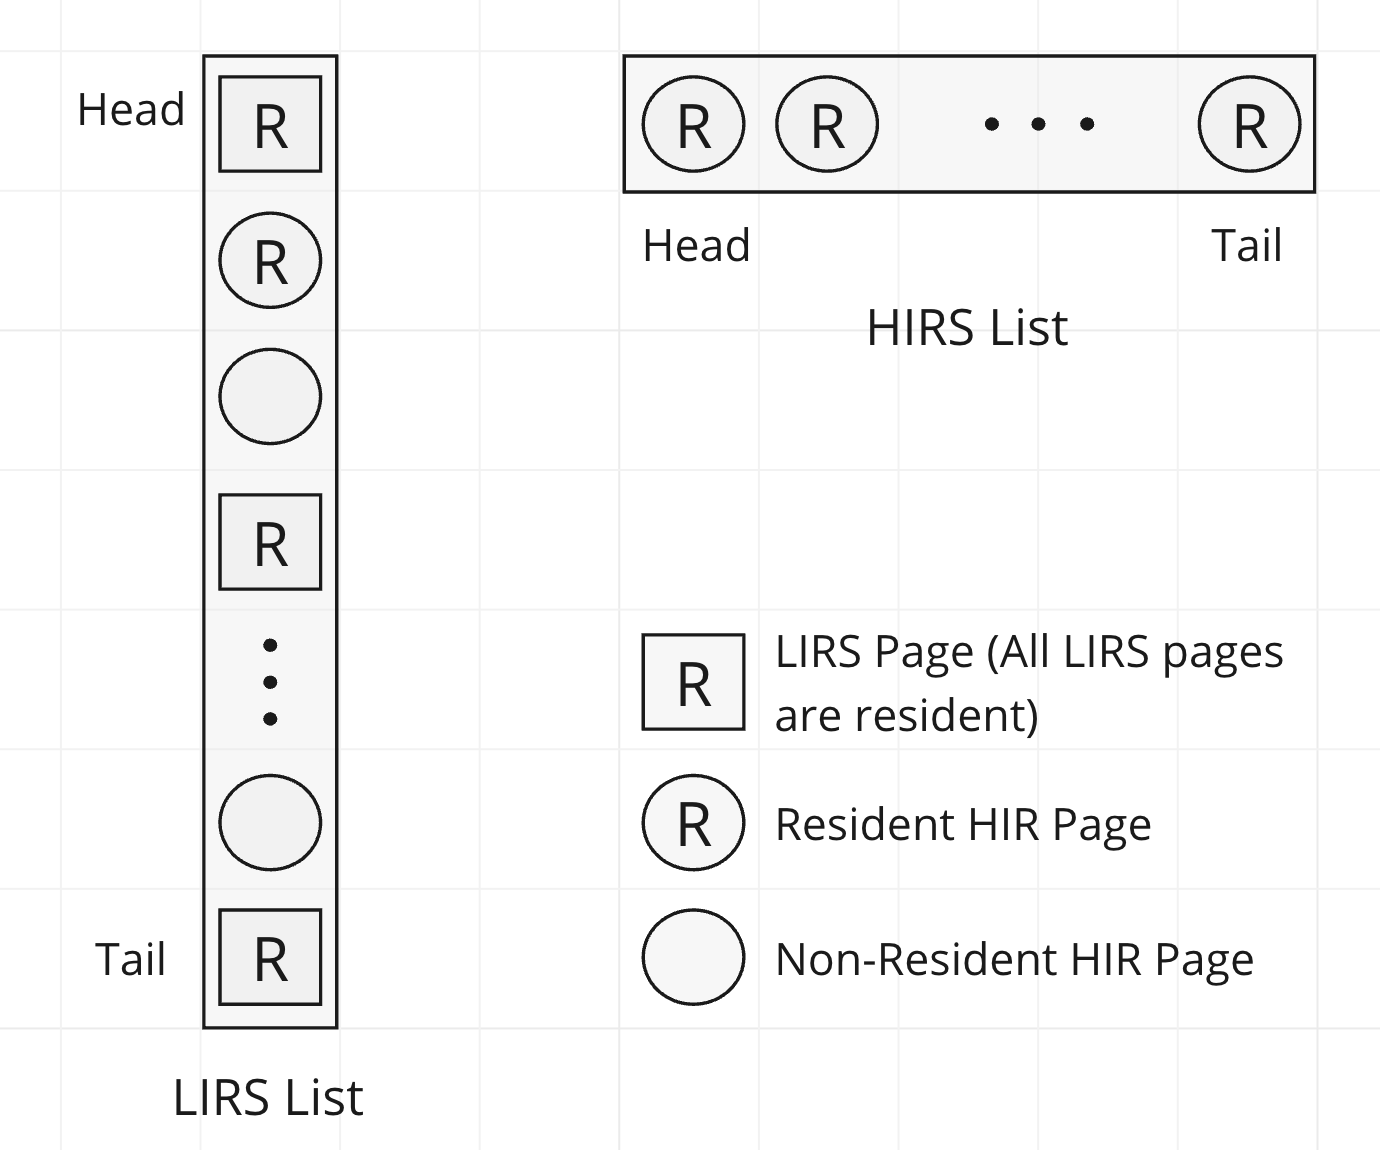
\includegraphics[width=\textwidth]{lirs_and_hirs_lists.png}
        \caption{LIRS and HIR lists}
        \label{fig:lirs_and_hirs_lists}
    \end{minipage}
    \hfill
\end{figure}

For LIRS cache, we can implement each of the functions as follows:

\begin{itemize}
    \item \textbf{UpdateAccessHistory}(\textit{page}, \textit{tenant}): If it is a LIR page, move it
    to the front of the LIRS list. If it is a HIR page that is on the LIRS list, it is recent, mark it 
    as a LIRS page, and move it to the front of the LIRS list. If it is a HIR page that is not on the LIRS
    list, it is not recent enough to be on the LIRS list, then add it to the front of the HIRS list, and 
    add it to the front of the LIRS list, but as a HIR page.
    \item \textbf{AddPageToCache}(\textit{page}, \textit{tenant}, \textit{buffer\_location}): If the page 
    is a non-resident HIR page that is in the LIRS list, move it to the front of the LIRS list, and make it a 
    LIRS page. If the page is not in the LIRS list, add it to the front of the LIRS and HIR lists, but mark it
    as a HIR page.
    \item \textbf{EvictPage}(\textit{tenant\_to\_evict}): If the HIRS list is not empty, evict the page from the 
    tail of the HIRS list, and update it in the LIRS list to mark it as non-resident HIR page. If the HIRS list is
    empty, evict the page from the tail of the LIRS list.
\end{itemize}

After each operation, we will prune the LIRS list if needed, and check if the tail of 
the LIRS list should be moved to the HIR list.

Each operation can be implemented in amortized $O(1)$ time, and the complexity overhead 
of LIRS is low \cite{lirs-article}.

\begin{figure}[htbp]
    \centering
    \begin{minipage}{\linewidth}
    \begin{algorithm}[H]
        \caption{LIRS Cache Eviction Policy}
        \begin{algorithmic}
            \STATE \textbf{function} UpdateAccessHistory(page, tenant):
            \STATE \hspace{\algorithmicindent} \textbf{if} LIRS\_Locations[tenant][page] != \textbf{null} \textbf{then}
            \STATE \hspace{\algorithmicindent} \hspace{\algorithmicindent} pageInLIRS = LIRS\_Locations[tenant][page]
            \STATE \hspace{\algorithmicindent} \hspace{\algorithmicindent} \textbf{if not} pageInLIRS.is\_LIR \textbf{then}
            \STATE \hspace{\algorithmicindent} \hspace{\algorithmicindent} \hspace{\algorithmicindent} pageInLIRS.is\_LIR = \textbf{true}
            \STATE \hspace{\algorithmicindent} \hspace{\algorithmicindent} \hspace{\algorithmicindent} pageInHirs = HIRS\_Locations[tenant][page]
            \STATE \hspace{\algorithmicindent} \hspace{\algorithmicindent} \hspace{\algorithmicindent} HIRS\_List[tenant].Remove(pageInHirs)
            \STATE \hspace{\algorithmicindent} \hspace{\algorithmicindent} \hspace{\algorithmicindent} HIRS\_Locations[tenant][page] = \textbf{null}
            \STATE \hspace{\algorithmicindent} \hspace{\algorithmicindent} \textbf{end if}
            \STATE \hspace{\algorithmicindent} \hspace{\algorithmicindent} LIRS\_List[tenant].\textbf{move\_to\_front}(page)
            \STATE \hspace{\algorithmicindent} \hspace{\algorithmicindent} LIRS\_Locations[tenant][page] = LIRS\_List[tenant].\textbf{head}
            \STATE \hspace{\algorithmicindent} \textbf{else}
            \STATE \hspace{\algorithmicindent} \hspace{\algorithmicindent} pageInHirs = HIRS\_Locations[tenant][page]
            \STATE \hspace{\algorithmicindent} \hspace{\algorithmicindent} HIRS\_List[tenant].\textbf{add\_to\_front}(page)
            \STATE \hspace{\algorithmicindent} \hspace{\algorithmicindent} HIRS\_Locations[tenant][page] = HIRS\_List[tenant].\textbf{head}
            \STATE \hspace{\algorithmicindent} \hspace{\algorithmicindent} LIRS\_List[tenant].\textbf{add\_to\_front}(page) \COMMENT {Marked as HIR}
            \STATE \hspace{\algorithmicindent} \hspace{\algorithmicindent} LIRS\_Locations[tenant][page] = LIRS\_List[tenant].\textbf{head}
            \STATE \hspace{\algorithmicindent} \textbf{end if}
            \STATE \textbf{end function}
            \STATE
            \STATE \textbf{function} AddPageToCache(page, tenant, buffer\_location):
            \STATE \hspace{\algorithmicindent} \textbf{if} LIRS\_Locations[tenant][page] != \textbf{null} \textbf{then}
            \STATE \hspace{\algorithmicindent} \hspace{\algorithmicindent} pageInLirs = LIRS\_Locations[tenant][page]
            \STATE \hspace{\algorithmicindent} \hspace{\algorithmicindent} pageInLirs.is\_LIR = \textbf{true}
            \STATE \hspace{\algorithmicindent} \hspace{\algorithmicindent} LIRS\_List[tenant].\textbf{move\_to\_front}(page)
            \STATE \hspace{\algorithmicindent} \hspace{\algorithmicindent} LIRS\_Locations[tenant][page] = LIRS\_List[tenant].\textbf{head}
            \STATE \hspace{\algorithmicindent} \textbf{else}
            \STATE \hspace{\algorithmicindent} \hspace{\algorithmicindent} HIRS\_List[tenant].\textbf{add\_to\_front}(page)
            \STATE \hspace{\algorithmicindent} \hspace{\algorithmicindent} HIRS\_Locations[tenant][page] = HIRS\_List[tenant].\textbf{head}
            \STATE \hspace{\algorithmicindent} \hspace{\algorithmicindent} LIRS\_List[tenant].\textbf{add\_to\_front}(page) \COMMENT {Marked as HIR}
            \STATE \hspace{\algorithmicindent} \hspace{\algorithmicindent} LIRS\_Locations[tenant][page] = LIRS\_List[tenant].\textbf{head}
            \STATE \hspace{\algorithmicindent} \textbf{end if}
            \STATE \textbf{end function}

            \STATE
            \STATE \textbf{function} EvictPage(tenant\_to\_evict):
            \STATE \hspace{\algorithmicindent} \textbf{if} \textbf{not} HIRS\_List[tenant\_to\_evict].\textbf{empty}() \textbf{then}
            \STATE \hspace{\algorithmicindent} \hspace{\algorithmicindent} pageInHirs = HIRS\_List[tenant\_to\_evict].\textbf{remove\_from\_tail}()
            \STATE \hspace{\algorithmicindent} \hspace{\algorithmicindent} HIRS\_Locations[tenant\_to\_evict][pageInHirs] = \textbf{null}
            \STATE \hspace{\algorithmicindent} \hspace{\algorithmicindent} \textbf{if} LIRS\_Locations[tenant\_to\_evict][pageInHirs] != \textbf{null} \textbf{then}
            \STATE \hspace{\algorithmicindent} \hspace{\algorithmicindent} \hspace{\algorithmicindent} pageInLirs = LIRS\_Locations[tenant\_to\_evict][pageInHirs]
            \STATE \hspace{\algorithmicindent} \hspace{\algorithmicindent} \hspace{\algorithmicindent} pageInLirs.is\_LIR = \textbf{false}
            \STATE \hspace{\algorithmicindent} \hspace{\algorithmicindent} \textbf{end if}
            \STATE \hspace{\algorithmicindent} \hspace{\algorithmicindent} \textbf{return} pageInHirs
            \STATE \hspace{\algorithmicindent} \textbf{else}
            \STATE \hspace{\algorithmicindent} \hspace{\algorithmicindent} pageInLirs = LIRS\_List[tenant\_to\_evict].\textbf{remove\_from\_tail}()
            \STATE \hspace{\algorithmicindent} \hspace{\algorithmicindent} LIRS\_Locations[tenant\_to\_evict][pageInLirs] = \textbf{null}
            \STATE \hspace{\algorithmicindent} \hspace{\algorithmicindent} \textbf{return} pageInLirs
            \STATE \hspace{\algorithmicindent} \textbf{end if}
            \STATE \textbf{end function}
        \end{algorithmic}
    \end{algorithm}
    \caption{LIRS Cache Eviction Policy}
    \label{fig:lirs}
    \end{minipage}
\end{figure}

\newpage

After each function, \textbf{UpdateAccessHistory}, \textbf{AddPageToCache}, and \textbf{EvictPage} 
finishes, we will call \textbf{PruneLIRSList}, and \textbf{MoveLIRSTailToHIRSIfNecessary} with the 
given tenant.

\begin{figure}[htbp]
    \centering
    \begin{minipage}{\linewidth}
    \begin{algorithm}[H]
        \begin{algorithmic}
            \STATE \textbf{function} PruneLIRSList(tenant):
            \STATE \hspace{\algorithmicindent} \textbf{while} \textbf{not} LIRS\_List[tenant].\textbf{empty}() \textbf{and} \textbf{not} LIRS\_List[tenant].\textbf{tail}.is\_LIR \textbf{do}
            \STATE \hspace{\algorithmicindent} \hspace{\algorithmicindent} pageInLirs = LIRS\_List[tenant].\textbf{remove\_from\_tail}()
            \STATE \hspace{\algorithmicindent} \hspace{\algorithmicindent} LIRS\_Locations[tenant][pageInLirs] = \textbf{null}
            \STATE \hspace{\algorithmicindent} \textbf{end while}
            \STATE \textbf{end function}
            \STATE
            \STATE \textbf{function} MoveLIRSTailToHIRSIfNecessary(tenant):
            \STATE \hspace{\algorithmicindent} tenantUsedCache = LIRS\_List[tenant].\textbf{number\_of\_LIRS\_pages}() + HIRS\_List[tenant].\textbf{size}()
            \STATE \hspace{\algorithmicindent} \textbf{if} LIRS\_List[tenant].\textbf{number\_of\_LIRS\_pages}() / tenantUsedCache $>$ LIRS\_Threshold \textbf{then}
            \STATE \hspace{\algorithmicindent} \hspace{\algorithmicindent} page = LIRS\_List[tenant].\textbf{remove\_from\_tail}()
            \STATE \hspace{\algorithmicindent} \hspace{\algorithmicindent} LIRS\_Locations[tenant][page] = \textbf{null}
            \STATE \hspace{\algorithmicindent} \hspace{\algorithmicindent} page.is\_LIR = \textbf{false}
            \STATE \hspace{\algorithmicindent} \hspace{\algorithmicindent} HIRS\_List[tenant].\textbf{add\_to\_front}(page)
            \STATE \hspace{\algorithmicindent} \hspace{\algorithmicindent} HIRS\_Locations[tenant][page] = HIRS\_List[tenant].\textbf{head}
            \STATE \hspace{\algorithmicindent} \hspace{\algorithmicindent} PruneLIRSList(tenant)
            \STATE \hspace{\algorithmicindent} \textbf{end if}
        \end{algorithmic}
    \end{algorithm}
    \caption{Helper Functions for LIRS Cache Eviction Policy}
    \label{fig:lirs-helper}
    \end{minipage}
\end{figure}

LIRS\_List is a doubly linked list that keeps the pages in the cache that are in the LIRS list.

LIRS\_Locations is a hash map or array that keeps the location of the pages in the LIRS list.

HIRS\_List is a doubly linked list that keeps the pages in the cache that are in the HIRS list.

HIRS\_Locations is a hash map or array that keeps the location of the pages in the HIRS list.

LIRS\_Threshold is a tunable parameter that defines the ratio of the number of LIRS pages with 
respect to the total number of pages in the cache.

In LIRS\_List, a counter of the number of LIRS pages is maintained, this counter is updated after 
each operation, and it is used allow $O(1)$ computation of \textbf{number\_of\_LIRS\_pages}()

\subsection{LRFU}

\subsection{Bélády Optimum (for comparison)}